\section{Sparsity Parameters for Graphs}
\label{sec:prelim-parameters}

\subsection{Parameterized Complexity and FPT}

This work uses parameterized algorithms, which leverage specific structural features of problem instances to achieve faster solutions. We present the essential definitions here; see~\cite[Chapter 2]{downey2013fundamentals} for comprehensive technical discussions.


\para{Parameterized Problem} We consider problems with multiple inputs, formalized as languages over two components. If a pair $\langle x, k \rangle$ belongs to such a language $L$, we call $k$ the parameter. The parameter typically takes integer values, though it may represent other structures such as graphs or algebraic objects. 



\para{Fixed-Parameter Tractability (FPT)~\cite{downey2013fundamentals}}
Formally, a parameterized language $L$ is \emph{fixed-parameter tractable} (FPT) if the following hold:
\begin{itemize}
    \item There exists an algorithm $\Phi$, a constant $c$, and a computable function $f$ such that for all instances $x, k$, $\Phi(\langle x, k \rangle)$ runs in time $f(k) \cdot |x|^c$,
    \item $\Phi(\langle x, k \rangle) = 1$ if and only if $\langle x, k \rangle \in L$.
\end{itemize}

Intuitively, this means that for each fixed value of the parameter $k$, the problem can be solved in polynomial time with respect to the input size $|x|$, where the degree of the polynomial does not depend on $k$. The potentially expensive part of the computation is isolated in the function $f(k)$, which can grow quickly, but for small $k$ the overall running time remains practical. This framework allows many NP-hard problems to become efficiently solvable when the parameter is small, even if the general problem is intractable.


\subsection{Treewidth}
\label{sec:prelim-parameters-treewidth}

The treewidth of a graph $G=(V, E)$ is defined via a \textit{tree decomposition}. A tree decomposition is a pair $(\mathcal{T}, \{X_i \mid i \in I\})$, where $\mathcal{T}=(I, F)$ is a tree and each $X_i$ (called a bag) is a subset of $V$, satisfying:
\begin{enumerate}
    \item The union of all bags equals $V$; i.e., $\bigcup_{i \in I} X_i = V$.
    \item For every edge $(u,v) \in E$, there is at least one bag $X_i$ containing both $u$ and $v$.
    \item For any vertex $v \in V$, the set of bags containing $v$ forms a connected subtree in $\mathcal{T}$.
\end{enumerate}


The \textit{width} of a tree decomposition is $\max_{i \in I} |X_i| - 1$. The \textit{treewidth} of a graph $G$, denoted $tw(G)$, is the minimum width over all possible tree decompositions of $G$. Figure~\ref{fig:prelim-tw} shows a graph and one of its tree decompositions. A low treewidth indicates a structure amenable to efficient dynamic programming, a property that we exploit extensively in Chapter~\ref{chp:hermes}.
\begin{figure}[h]
    \centering
    \begin{minipage}{0.48\textwidth}
        \centering
        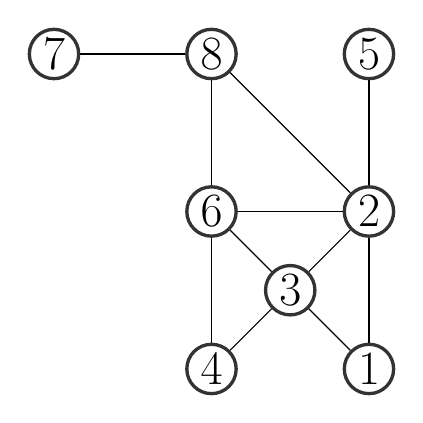
\begin{tikzpicture}[
  every node/.style={circle, draw=black!80, very thick, inner sep=1.5pt, font=\LARGE, fill=white, text=black},
  every path/.style={}
]
  \node (v8) at (0,4) {8};
  \node (v7) at (-2,4) {7};
  \node (v5) at (2,4) {5};
  \node (v6) at (0,2) {6};
  \node (v2) at (2,2) {2};
  \node (v4) at (0,0) {4};
  \node (v1) at (2,0) {1};
  \node (v3) at (1,1) {3};
  \draw (v1) -- (v2);
  \draw (v1) -- (v3);
  \draw (v2) -- (v3);
  \draw (v2) -- (v5);
  \draw (v2) -- (v6);
  \draw (v2) -- (v8);
  \draw (v3) -- (v4);
  \draw (v3) -- (v6);
  \draw (v4) -- (v6);
  \draw (v6) -- (v8);
  \draw (v7) -- (v8);
\end{tikzpicture}

        \caption*{(a) Example graph}
    \end{minipage}\hfill
    \begin{minipage}{0.48\textwidth}
        \centering
        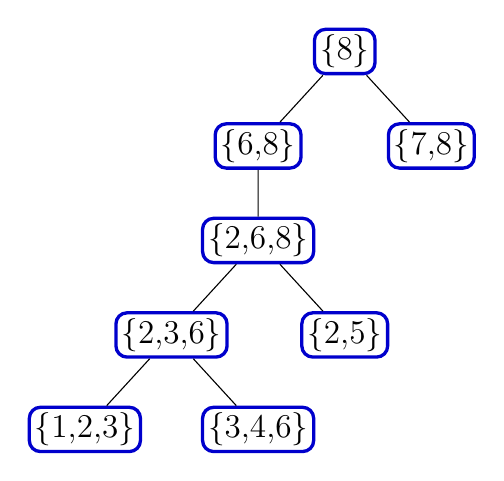
\begin{tikzpicture}[
  grow=down, level distance=12mm, sibling distance=22mm,
  every node/.style={draw=blue!80!black, very thick, rounded corners, font=\large, align=center, inner sep=2pt, fill=white, text=black}
]
  \node (b7) {\{8\}} child {node (b5) {\{6,8\}} child {node (b4) {\{2,6,8\}} child {node (b2) {\{2,3,6\}} child {node (b0) {\{1,2,3\}}} child {node (b1) {\{3,4,6\}}}} child {node (b3) {\{2,5\}}}}} child {node (b6) {\{7,8\}}};
\end{tikzpicture}

        \caption*{(b) Tree decomposition}
    \end{minipage}
    \caption{A graph and one of its tree decompositions~\cite{goharshady2023efficient}.}
    \label{fig:prelim-tw}
\end{figure}


\subsection{Pathwidth}
\label{sec:prelim-parameters-pathwidth}
A \emph{path decomposition} of a graph $G = (V, E)$ is a tree decomposition $(\mathcal{T}, \{X_i \mid i \in I\})$ where the tree $\mathcal{T}$ is a path. The \emph{width} of a path decomposition is $\max_{i \in I} |X_i| - 1$, as in the case of treewidth~\cite{conrado2023bounded, robertson1983graph}. 

\begin{figure}[h]
    \centering
    \begin{minipage}{0.8\textwidth}
        \centering
        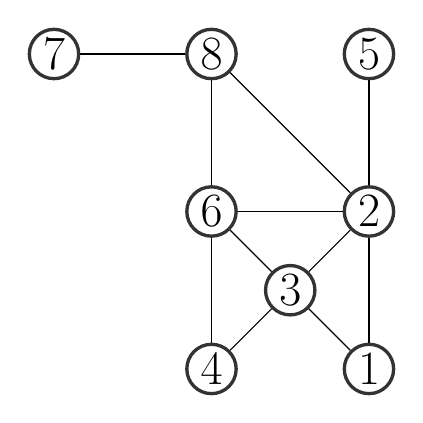
\begin{tikzpicture}[
  every node/.style={circle, draw=black!80, very thick, inner sep=1.5pt, font=\LARGE, fill=white, text=black},
  every path/.style={}
]
  \node (v8) at (0,4) {8};
  \node (v7) at (-2,4) {7};
  \node (v5) at (2,4) {5};
  \node (v6) at (0,2) {6};
  \node (v2) at (2,2) {2};
  \node (v4) at (0,0) {4};
  \node (v1) at (2,0) {1};
  \node (v3) at (1,1) {3};
  \draw (v1) -- (v2);
  \draw (v1) -- (v3);
  \draw (v2) -- (v3);
  \draw (v2) -- (v5);
  \draw (v2) -- (v6);
  \draw (v2) -- (v8);
  \draw (v3) -- (v4);
  \draw (v3) -- (v6);
  \draw (v4) -- (v6);
  \draw (v6) -- (v8);
  \draw (v7) -- (v8);
\end{tikzpicture}

        \caption*{(a) Example graph}
    \end{minipage}
    
    \vspace{1em}
    
    \begin{minipage}{0.8\textwidth}
        \centering
        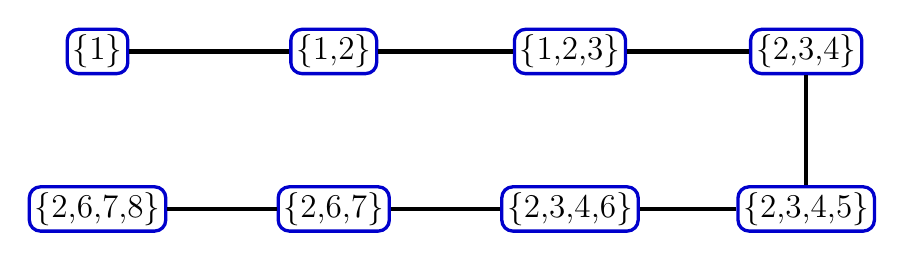
\begin{tikzpicture}[
  every node/.style={draw=blue!80!black, very thick, rounded corners, font=\large, align=center, inner sep=2pt, fill=white, text=black},
  every path/.style={}
]
  % Snake layout for better fit
  % Snake layout: top row then bottom row
  \node (p0) at (0.0,0) {\{1\}};
  \node (p1) at (3.0,0) {\{1,2\}};
  \draw[line width=1.5pt] (p0) -- (p1);
  \node (p2) at (6.0,0) {\{1,2,3\}};
  \draw[line width=1.5pt] (p1) -- (p2);
  \node (p3) at (9.0,0) {\{2,3,4\}};
  \draw[line width=1.5pt] (p2) -- (p3);

  \node (p4) at (9.0,-2.0) {\{2,3,4,5\}};
  \draw[line width=1.5pt] (p3) -- (p4);
  \node (p5) at (6.0,-2.0) {\{2,3,4,6\}};
  \draw[line width=1.5pt] (p4) -- (p5);
  \node (p6) at (3.0,-2.0) {\{2,6,7\}};
  \draw[line width=1.5pt] (p5) -- (p6);
  \node (p7) at (0.0,-2.0) {\{2,6,7,8\}};
  \draw[line width=1.5pt] (p6) -- (p7);
\end{tikzpicture}

        \caption*{(b) Path decomposition}
    \end{minipage}
    \caption{A graph and one of its path decompositions~\cite{goharshady2023efficient}.}
    \label{fig:prelim-pw}
\end{figure}

Intuitively, pathwidth measures how similar a graph is to a path: a lower pathwidth means the graph can be decomposed into a sequence of overlapping vertex sets (bags) with limited size, capturing the "path-like" structure of the graph. Pathwidth is always at least as large as treewidth, since every path decomposition is also a tree decomposition.



\subsection{Treedepth Decomposition}
\label{sec:prelim-parameters-treedepth}

For a graph $G= (V, E),$ a \emph{treedepth decomposition}~\cite{nevs2012bounded, iwata2017power, nevs2015low} is a rooted tree $T = (V, E_T)$ on the same set of vertices as $G$ that satisfies the following requirement:
\begin{itemize}
	\item For every undirected edge $\{u, v\} \in E$ or directed edge $(u, v) \in E$ of the original graph, either $u$ is an ancestor of $v$ in $T$ or $v$ is an ancestor of $u$ in $T.$
\end{itemize}

We say that a treedepth decomposition $T$ is optimal if it has the smallest possible depth among all decompositions of $G.$ This smallest depth is called the \emph{treedepth} of $G.$ Intuitively, treedepth is a measure of graph sparsity that captures how much a graph resembles a shallow tree. Figure~\ref{fig:prelim-tdp} shows a graph and one of its treedepth decompositions.

\begin{figure}[h]
    \centering
    \begin{minipage}{0.48\textwidth}
        \centering
        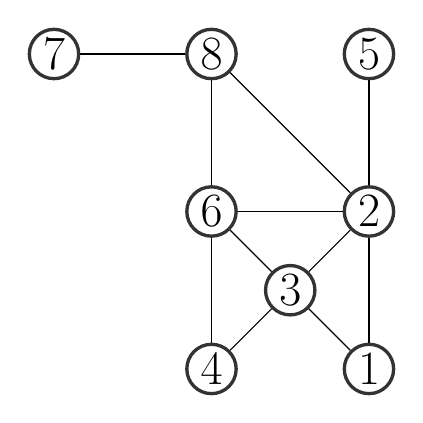
\begin{tikzpicture}[
  every node/.style={circle, draw=black!80, very thick, inner sep=1.5pt, font=\LARGE, fill=white, text=black},
  every path/.style={}
]
  \node (v8) at (0,4) {8};
  \node (v7) at (-2,4) {7};
  \node (v5) at (2,4) {5};
  \node (v6) at (0,2) {6};
  \node (v2) at (2,2) {2};
  \node (v4) at (0,0) {4};
  \node (v1) at (2,0) {1};
  \node (v3) at (1,1) {3};
  \draw (v1) -- (v2);
  \draw (v1) -- (v3);
  \draw (v2) -- (v3);
  \draw (v2) -- (v5);
  \draw (v2) -- (v6);
  \draw (v2) -- (v8);
  \draw (v3) -- (v4);
  \draw (v3) -- (v6);
  \draw (v4) -- (v6);
  \draw (v6) -- (v8);
  \draw (v7) -- (v8);
\end{tikzpicture}

        \caption*{(a) Example graph}
    \end{minipage}\hfill
    \begin{minipage}{0.48\textwidth}
        \centering
        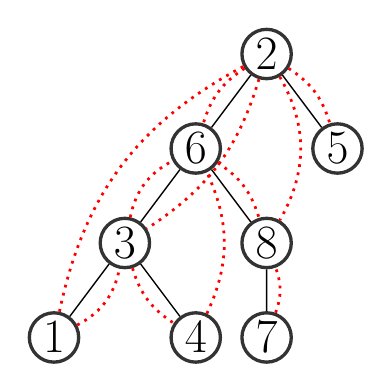
\begin{tikzpicture}[
  grow=down, level distance=12mm, sibling distance=18mm,
  every node/.style={circle, draw=black!80, very thick, inner sep=1.5pt, font=\LARGE, fill=white, text=black},
  edge from parent/.style={draw, line width=0.5pt}
]
  \node (t2) {2} child {node (t6) {6} child {node (t3) {3} child {node (t1) {1}} child {node (t4) {4}}} child {node (t8) {8} child {node (t7) {7}}}} child {node (t5) {5}};
  % original graph edges (dotted, now red and curvy)
  \draw[dotted, red, line width=1pt, bend left=25] (t1) to (t2);
  \draw[dotted, red, line width=1pt, bend right=25] (t1) to (t3);
  \draw[dotted, red, line width=1pt, bend left=20] (t2) to (t3);
  \draw[dotted, red, line width=1pt, bend left=20] (t2) to (t5);
  \draw[dotted, red, line width=1pt, bend right=20] (t2) to (t6);
  \draw[dotted, red, line width=1pt, bend left=30] (t2) to (t8);
  \draw[dotted, red, line width=1pt, bend right=20] (t3) to (t4);
  \draw[dotted, red, line width=1pt, bend left=25] (t3) to (t6);
  \draw[dotted, red, line width=1pt, bend right=25] (t4) to (t6);
  \draw[dotted, red, line width=1pt, bend left=20] (t6) to (t8);
  \draw[dotted, red, line width=1pt, bend right=20] (t7) to (t8);
\end{tikzpicture}

        \caption*{(b) Treedepth decomposition}
    \end{minipage}
    \caption{A graph and one of its treedepth decompositions~\cite{goharshady2023efficient}.}
    \label{fig:prelim-tdp}
\end{figure}

For any small fixed $d,$ there is an algorithm that decides whether an input graph has treedepth $d$ in linear time and if so, outputs an optimal treedepth decomposition~\cite{reidl2014faster}. There are also well-optimized tools and libraries for computing treedepth decompositions~\cite{strasser2020pace}. 



